\chapter{Meta-Trained Transformers}\label{ch:networks}

The Bayes-optimal predictor of Chapters~\ref{ch:specificity} and~\ref{ch:reliability} knows how specific and how reliable descriptions are. A network must instead learn both properties from its training data. In this chapter, we meta-train Transformers (Section~\ref{sec:bg-bayes}) on the setting of Chapter~\ref{ch:setup} and ask two questions. How close do the networks come to the Bayes-optimal ESS? And what sets how much they trust a description?

\section{Setup}\label{sec:net-setup}
\paragraph{Networks.} We encode prompts with the prefix embedding of \citet{huangge2025}. A prompt consists of an optional description token that carries $m$, up to $20$ demonstration tokens, and a query token. The network is a Transformer \citep{vaswani2017} of the same size as that of \citet{garg2022} ($12$ layers, $8$ heads, and width $256$) and is trained with their optimizer. Unlike theirs, it uses bidirectional attention and no positional encoding (Section~\ref{sec:training}). To keep training short, we use $d = 5$, with $a_0 = 10$ as before. The network outputs a mean and a log variance for the query's label and is trained with log loss, as in \citet{zhu2026}. The mean that minimizes this loss is the posterior mean, which is the Bayes-optimal prediction under squared error. We therefore score the network's mean by its squared error~\eqref{eq:regret}, the same error that we use for the Bayes-optimal predictor. The description token carries only $m$, and half of the training prompts omit it, so each network must learn $r$ and $p$ from its training distribution. We train a network for each combination of specificity ($r = 0.1$, loose; $r = 0.01$, specific) and reliability ($p \in \{1, 0.99, 0.9\}$). For each specific setting, we train three networks that differ only in their random seed. For each loose setting, we train two. Section~\ref{sec:training} describes four further networks, at $r = 0.5$ and $r = 0.05$.

\paragraph{Evaluation.} We test each network on $20{,}000$ fresh prompts at every $n$ from $0$ to $20$, with and without a description. Networks that differ only in their seed are tested on the same prompts. Each network is tested at its training reliability and at $p = 1$ and $p = 0.9$. The networks trained with the second and third seeds are also tested at $p = 0.99$ (Table~\ref{tab:networks}). We read each network's ESS from its own error curves, following Definition~\ref{def:ess}. Without a description, the networks' errors are close to the Bayes-optimal predictor's. At $n = 0$, where the Bayes-optimal error is about $50$, every network's error is within $0.21$ of it. Averaged over the numbers of demonstrations on which a network was trained, the difference is at most $0.3$.

We compare each network's ESS with that of two Bayes-optimal predictors. The \emph{trained} Bayes-optimal predictor uses the reliability on which the network was trained. The \emph{calibrated} Bayes-optimal predictor uses the reliability of the test prompts. Finally, to summarize how much a network trusts a description, we define its \emph{implied trust}. With no demonstrations, the Bayes-optimal prediction at reliability $q$ is $q\, m^\top x$. A network's implied trust is the value of $q$ for which this prediction is closest to the network's prediction in squared error. It equals the regression coefficient of the network's prediction on $m^\top x$, and it can exceed $1$ (Table~\ref{tab:networks}).

\begin{figure}[t]
\centering
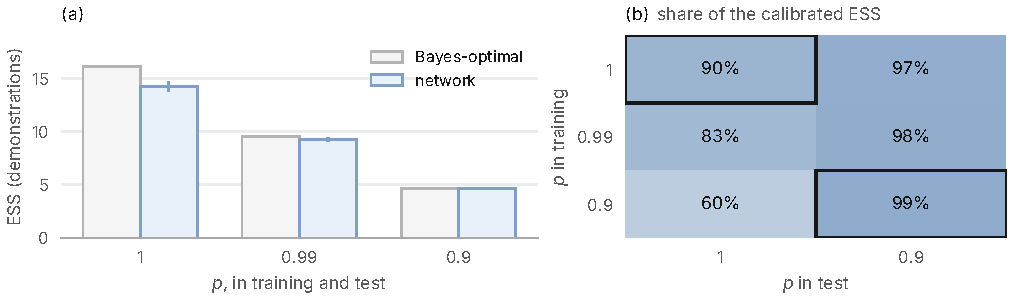
\includegraphics[width=\textwidth]{networks.pdf}
\caption[The ESS of a description to meta-trained networks]{\textbf{Networks come close to the Bayes-optimal ESS and take their trust in a description from training.} All panels use the specific description ($r = 0.01$), $d = 5$, $a_0 = 10$, and no demonstrations. Each network ESS shown is the mean over three networks trained with different random seeds, and the error bars show $\pm$ one standard deviation across them. (a) Networks trained and tested at the same reliability $p$. The bars show the Bayes-optimal ESS on the same prompts and the network's ESS, which is read from the network's own no-description curve. (b) Networks trained at one reliability and tested at another. Each cell shows the network's ESS as a share of the calibrated predictor's, and outlined cells mark cases where the training and test reliabilities match. Table~\ref{tab:networks} gives every value, including those for the loose description ($r = 0.1$).}
\label{fig:networks}
\end{figure}

\section{Results}\label{sec:net-results}
\paragraph{Networks come close to the Bayes-optimal ESS.} We first train and test each network at the same reliability (Figure~\ref{fig:networks}a). For the specific description at $p = 1$, the network's ESS is $14.3 \pm 0.5$ (mean $\pm$ standard deviation over three seeds). On the same prompts, the Bayes-optimal ESS is $16.1$. On $200{,}000$ prompts, it is $15.9$, close to the value $c + d + 1 = 16$ of Theorem~\ref{thm:reliable}(ii), since $c = 1/(r a_0) = 10$. At $p = 0.99$, the network's ESS is $9.3 \pm 0.2$, compared with $9.6$ for the Bayes-optimal predictor on the same prompts. At $p = 0.9$, it is $4.66 \pm 0.01$, compared with $4.63$. Because the three networks share their test prompts, these standard deviations reflect training alone and leave out the variation from prompts. We therefore compare each network with the Bayes-optimal predictor on the same prompts. Table~\ref{tab:networks} instead gives the Bayes-optimal ESS on $200{,}000$ prompts. At $p = 0.99$, that value ($8.96$) lies below the networks' mean ESS, whereas the Bayes-optimal ESS on the networks' own prompts ($9.6$) lies above it. A network's ESS can exceed the Bayes-optimal ESS on the same prompts, as it does at $p = 0.9$, because it is read from the network's own no-description curve rather than from the Bayes-optimal one. For the loose description, the network's ESS is within $0.1$ of the Bayes-optimal ESS at every reliability. At $p = 1$, for example, it is $5.85 \pm 0.03$, compared with $5.89$ (Table~\ref{tab:networks}).

\paragraph{ESS as demonstrations accumulate.} Figure~\ref{fig:networks-ess-n} shows each network's $\ess_n$ at its training reliability as demonstrations accumulate. The test prompts hold at most $20$ demonstrations, so the largest $\ess_n$ that can be read is $20 - n$. For the loose description, the networks' $\ess_n$ follows the Bayes-optimal $\ess_n$ to within $0.6$ at every $n$ the grid can show. For the specific description, the networks fall short of the Bayes-optimal $\ess_n$ by up to $2.4$ demonstrations at $p = 1$, $2.9$ at $p = 0.99$, and $1.4$ at $p = 0.9$. They exceed it by at most $0.3$. Both comparisons hold until the ESS can no longer be read within the grid. With five demonstrations in hand, the three networks trained at $p = 0.9$ have an ESS of $4.83$, $4.79$, and $4.77$, compared with $5.20$ for the Bayes-optimal predictor.

\begin{figure}[t]
\centering
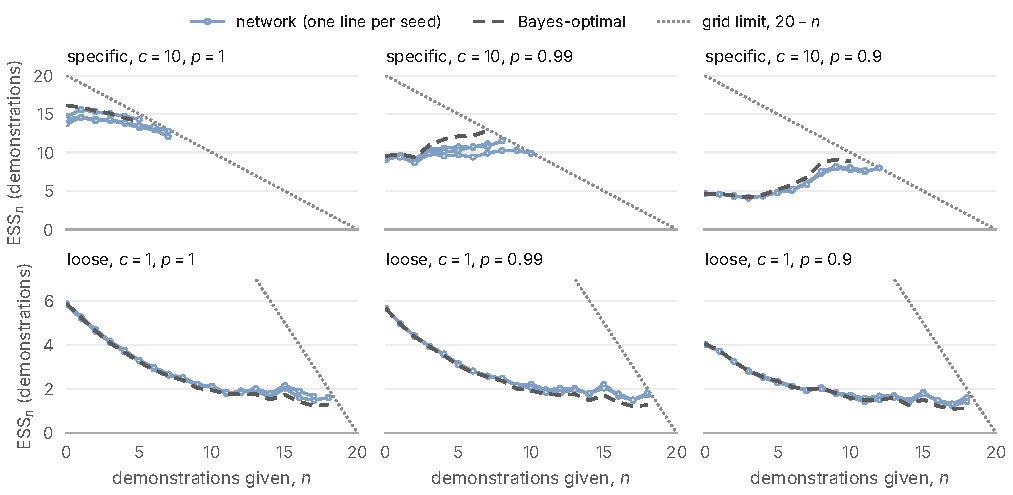
\includegraphics[width=\textwidth]{networks_ess_n.pdf}
\caption[The networks' ESS as demonstrations accumulate]{\textbf{The networks' ESS as demonstrations accumulate.} Each panel shows $\ess_n$ for the meta-trained networks, with one line per training seed, and for the Bayes-optimal predictor on the same prompts. The networks are trained and tested at the same reliability $p$. The top row uses the specific description ($r = 0.01$), and the bottom row uses the loose description ($r = 0.1$). Here $d = 5$ and $a_0 = 10$, and each network is tested on $20{,}000$ prompts. A curve stops where the error without the description would reach the error with it only after more than the $20$ demonstrations of the grid. The dotted line, $20 - n$, is the largest ESS that the grid can show.}
\label{fig:networks-ess-n}
\end{figure}

\paragraph{Training sets a network's trust.} With no demonstrations, the prompt carries no information about relevance (Section~\ref{sec:proof-unreliable}, Step~1). Any learner must therefore take its trust in a description from its training. The networks show how much of that trust they take (Figure~\ref{fig:networks}b). The networks trained at $p = 0.9$ keep hedging even when every test description is relevant. Their implied trust is $0.87$ to $0.89$ across the three seeds. Their ESS on reliable descriptions is $9.5 \pm 0.4$, whereas the calibrated predictor reaches $15.9$ and the trained one $10.8$.

The networks trained on specific descriptions at $p = 1$ or $p = 0.99$ treat every description as relevant when no demonstrations are shown. Their implied trust lies between $0.95$ and $1.02$, so the two training reliabilities cannot be told apart without demonstrations. Demonstrations separate them. On prompts in which one description in ten is irrelevant, the description lowers the error of the networks trained at $p = 0.99$ at every $n$, as it does for the Bayes-optimal predictor. It lowers their error by $3.5$ to $3.7$ with six demonstrations and by $0.08$ to $0.13$ with $20$. The networks trained at $p = 1$ instead trust the description fully. As Section~\ref{sec:trust} predicts, full trust costs little with no demonstrations. Their ESS is then $4.58 \pm 0.03$, compared with $4.70$ for the calibrated predictor. From six demonstrations on, however, their error is higher with the description than without it, in all three seeds. The fully trusting Bayes-optimal predictor behaves in the same way. With eight demonstrations, for example, the first of these networks has an error of $4.6$ with the description and $2.3$ without it.

\begin{table}[t]
\centering\small
\caption[The meta-trained networks against the Bayes-optimal predictors]{\textbf{The meta-trained networks against the Bayes-optimal predictors.} Here $d = 5$ and $a_0 = 10$, and each network is evaluated on $20{,}000$ prompts. Rows are grouped by training reliability, and ``Seeds'' gives the number of networks, trained with different random seeds, behind each row. ``Network'' is the mean ESS over these networks, $\pm$ the standard deviation across them; for a single network, it is $\pm$ the standard error over prompts. ``Trained'' and ``calibrated'' are the Bayes-optimal predictors that use the training and the test reliability, respectively, and they are shown once where the two coincide. Calibrated values, and trained values where the two reliabilities coincide, use $200{,}000$ prompts (standard errors at most $0.1$). Other trained values use the network's evaluation prompts. Prompt noise alone can move these values by up to $0.6$, so a trained value can exceed the calibrated one. ``Trust'' is the network's implied trust with no demonstrations, averaged over the networks in the row.}
\label{tab:networks}
\vspace{3pt}
\begin{tabular}{rrrcrrrr}
\toprule
& & & & \multicolumn{3}{c}{ESS} & \\
\cmidrule(lr){5-7}
$r$ & $p_{\mathrm{train}}$ & $p_{\mathrm{test}}$ & Seeds & Network & Trained & Calibrated & Trust \\
\midrule
0.1 & 1 & 1 & 2 & 5.85 $\pm$ 0.03 & 5.89 & --- & 0.964 \\
0.1 & 1 & 0.99 & 1 & 5.65 $\pm$ 0.06 & 5.66 & 5.61 & 0.991 \\
0.1 & 1 & 0.9 & 2 & 4.02 $\pm$ 0.03 & 3.98 & 4.10 & 0.964 \\
0.01 & 1 & 1 & 3 & 14.26 $\pm$ 0.48 & 15.91 & --- & 1.008 \\
0.01 & 1 & 0.99 & 2 & 9.38 $\pm$ 0.16 & 9.54 & 8.96 & 1.015 \\
0.01 & 1 & 0.9 & 3 & 4.58 $\pm$ 0.03 & 4.54 & 4.70 & 1.008 \\
\midrule
0.1 & 0.99 & 1 & 2 & 5.87 $\pm$ 0.01 & 5.88 & 5.89 & 0.963 \\
0.1 & 0.99 & 0.99 & 2 & 5.65 $\pm$ 0.01 & 5.61 & --- & 0.963 \\
0.1 & 0.99 & 0.9 & 2 & 4.02 $\pm$ 0.03 & 3.99 & 4.10 & 0.963 \\
0.01 & 0.99 & 1 & 3 & 13.28 $\pm$ 0.57 & 16.01 & 15.91 & 0.982 \\
0.01 & 0.99 & 0.99 & 3 & 9.25 $\pm$ 0.15 & 8.96 & --- & 0.982 \\
0.01 & 0.99 & 0.9 & 3 & 4.60 $\pm$ 0.04 & 4.56 & 4.70 & 0.982 \\
\midrule
0.1 & 0.9 & 1 & 2 & 5.67 $\pm$ 0.06 & 5.75 & 5.89 & 0.883 \\
0.1 & 0.9 & 0.99 & 1 & 5.51 $\pm$ 0.06 & 5.55 & 5.61 & 0.901 \\
0.1 & 0.9 & 0.9 & 2 & 4.03 $\pm$ 0.01 & 4.10 & --- & 0.883 \\
0.01 & 0.9 & 1 & 3 & 9.49 $\pm$ 0.44 & 10.79 & 15.91 & 0.876 \\
0.01 & 0.9 & 0.99 & 2 & 8.08 $\pm$ 0.28 & 8.55 & 8.96 & 0.880 \\
0.01 & 0.9 & 0.9 & 3 & 4.66 $\pm$ 0.01 & 4.70 & --- & 0.876 \\
\bottomrule
\end{tabular}

\end{table}

\section{Training Details}\label{sec:training}
Each demonstration token holds an input together with its label, and two indicator coordinates mark the token type. There is no positional encoding. The Transformer has $12$ layers, $8$ heads, and width $256$. It is trained with Adam (learning rate $10^{-4}$) for $40{,}000$ steps at batch size $1{,}024$, on fresh prompts at every step and without a curriculum. When a prompt has no description, the description token is masked out of attention. The prediction is read at the query token. The labels and the description are divided by $\sqrt{a_0}$ before they enter the network. Gradients are clipped to norm $1$, and training uses bfloat16 autocast. The number of demonstrations in a training prompt is uniform on $0$ to $20$ ($0$ to $15$ for the $r = 0.05$ and $r = 0.5$ networks described below).

Four further networks were trained once each, at $r = 0.5$ ($p = 1$ and $p = 0.9$) and at $r = 0.05$ ($p = 1$ and $p = 0.9$). Each reaches an ESS within $0.03$ of the Bayes-optimal ESS. The four values are $2.64$ compared with $2.66$, $2.16$ compared with $2.15$, $7.32$ compared with $7.35$, and $4.38$ compared with $4.37$.
